\section{Methology}

Rendering images is usually achieved by casting a set amount of rays onto a 3D object and calculating all intersection points.
Once an intersection is found a ray may spawn one or more rays at the intersection point in order to simulate effects such as reflections, glossy surfaces, semi-transparent materials, etc.
It is also possible that no intersection is found if the ray leaves the bounding box. This is the equivalent of a ray "shooting into the sky".
These rays do not contribute to the result and are usually discarded. 
Since the exact point of exit is not required and no additional rays are spawned theses rays are cheaper to compute.


\begin{figure}[H]
	\centering
	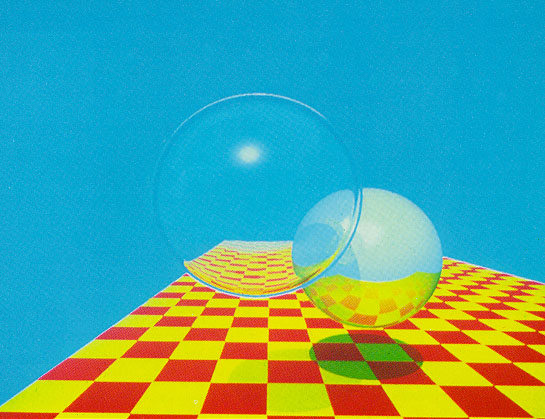
\includegraphics[width=0.75\textwidth]{res/rendered_image_turner.png}
	\caption{One of the first rendered digitally rendered images \cite{rendering_turner}. From the observer's eye about half represents the sky. Rays casted there can be discarded}
	\label{fig::nvidia_benchmark}
\end{figure}


The main difference between image rendering and applications in Semiconductor Process Simulation is that there are usually no skyboxes.
Furthermore it is undesireable to discard rays since they do not contribute to the simulation and are therefore wasted computing power.


